\documentclass[11pt]{article}

% Language setting
\usepackage[turkish]{babel}
\usepackage{pythonhighlight}

\usepackage[a4paper,top=2cm,bottom=2cm,left=2cm,right=2cm,marginparwidth=2cm]{geometry}

% Useful packages
\usepackage{amsmath}
\usepackage{graphicx}
\usepackage[colorlinks=true, allcolors=blue]{hyperref}
\usepackage{verbatim}
\usepackage{fancyhdr} % for header and footer
\usepackage{titlesec}
\usepackage{parskip}

\setlength{\parindent}{0pt}

\titleformat{\subsection}[runin]{\bfseries}{\thesubsection}{1em}{}

\pagestyle{fancy} % activate the custom header/footer

% define the header/footer contents
\lhead{\small{23BLM-4014 Yapay Sinir Ağları Ara Sınav Soru ve Cevap Kağıdı}}
\rhead{\small{Dr. Ulya Bayram}}
\lfoot{}
\rfoot{}

% remove header/footer on first page
\fancypagestyle{firstpage}{
  \lhead{}
  \rhead{}
  \lfoot{}
  \rfoot{\thepage}
}
 

\title{Çanakkale Onsekiz Mart Üniversitesi, Mühendislik Fakültesi, Bilgisayar Mühendisliği Akademik Dönem 2022-2023\\
Ders: BLM-4014 Yapay Sinir Ağları/Bahar Dönemi\\ 
ARA SINAV SORU VE CEVAP KAĞIDI\\
Dersi Veren Öğretim Elemanı: Dr. Öğretim Üyesi Ulya Bayram}
\author{%
\begin{minipage}{\textwidth}
\raggedright
Öğrenci Adı Soyadı: Mustafa Ozan Çetin\\ % Adınızı soyadınızı ve öğrenci numaranızı noktaların yerine yazın
Öğrenci No: 190401009
\end{minipage}%
}

\date{14 Nisan 2023}

\begin{document}
\maketitle

\vspace{-.5in}
\section*{Açıklamalar:}
\begin{itemize}
    \item Vizeyi çözüp, üzerinde aynı sorular, sizin cevaplar ve sonuçlar olan versiyonunu bu formatta PDF olarak, Teams üzerinden açtığım assignment kısmına yüklemeniz gerekiyor. Bu bahsi geçen PDF'i oluşturmak için LaTeX kullandıysanız, tex dosyasının da yer aldığı Github linkini de ödevin en başına (aşağı url olarak) eklerseniz bonus 5 Puan! (Tavsiye: Overleaf)
    \item Çözümlerde ya da çözümlerin kontrolünü yapmada internetten faydalanmak, ChatGPT gibi servisleri kullanmak serbest. Fakat, herkesin çözümü kendi emeğinden oluşmak zorunda. Çözümlerinizi, cevaplarınızı aşağıda belirttiğim tarih ve saate kadar kimseyle paylaşmayınız. 
    \item Kopyayı önlemek için Github repository'lerinizin hiçbirini \textbf{14 Nisan 2023, saat 15:00'a kadar halka açık (public) yapmayınız!} (Assignment son yükleme saati 13:00 ama internet bağlantısı sorunları olabilir diye en fazla ekstra 2 saat daha vaktiniz var. \textbf{Fakat 13:00 - 15:00 arası yüklemelerden -5 puan!}
    \item Ek puan almak için sağlayacağınız tüm Github repository'lerini \textbf{en geç 15 Nisan 2023 15:00'da halka açık (public) yapmış olun linklerden puan alabilmek için!}
    \item \textbf{14 Nisan 2023, saat 15:00'dan sonra gönderilen vizeler değerlendirilmeye alınmayacak, vize notu olarak 0 (sıfır) verilecektir!} Son anda internet bağlantısı gibi sebeplerden sıfır almayı önlemek için assignment kısmından ara ara çözümlerinizi yükleyebilirsiniz yedekleme için. Verilen son tarih/saatte (14 Nisan 2023, saat 15:00) sistemdeki en son yüklü PDF geçerli olacak.
    \item Çözümlerin ve kodların size ait ve özgün olup olmadığını kontrol eden bir algoritma kullanılacaktır. Kopya çektiği belirlenen vizeler otomatikman 0 (sıfır) alacaktır. Bu nedenle çözümlerinizi ve kodlarınızı yukarıda sağladığım gün ve saatlere kadar kimseyle paylaşmayınız.
    \item Bu vizeden alınabilecek en yüksek not 100'dür. Toplam aldığınız puan 100'ü geçerse, aldığınız not 100'e sabitlenecektir.
    \item LaTeX kullanarak PDF oluşturanlar öz geçmişlerine LaTeX bildiklerini de eklemeyi unutmasınlar :)
    \item Bu vizedeki soruların çözümleri ve tex dosyası için istediğiniz kadar sayıda Github repository'si oluşturabilirsiniz. Sadece yukarıda belirttiğim tarihlerde (14 Nisan 2023 saat 15:00 ile 15 Nisan 2023 saat 15:00 arasında) public yapmayı/halka açmayı ve Github profilinizi de öz geçmişinize eklemeyi unutmayın :)
    \item Bilgisayarınıza hiçbir program kurmadan, Overleaf, Google Colab, Kaggle gibi ortamlar üzerinden bu vizeyi tamamlamanız mümkün. İyi çalışmalar!!
\end{itemize}

(Ekstra 5 puan) \url{https://github.com/mozancetin/Yapay-Sinir-Aglari/blob/main/main.tex}

\newpage
\section{(Toplam 10 Puan) Hopfield Networks:}

\subsection{(2 Puan)} \textbf{ChatGPT’ye size Hopfield Network’ler ile ilgili detaylı bilgi vermesini isteyin. Sorduğunuz soruyu, ChatGPT'nin çıkartığı cevabı aşağı koyun. Bu cevapta anlamadığınız terimleri de ChatGPT’ye sorup, sorduğunuz soruları ve ChatGPT’nin verdiği cevapları da sırayla aşağı koyun.}

\textbf{Soru:} 
Hopfield Network'ler hakkında detaylı bilgi verebilir misin?

\textbf{Cevap (ChatGPT):}
Elbette! Hopfield Network, yapay sinir ağlarının bir türüdür ve özellikle bellek ve hatırlama sorunları için kullanılır. İsmini, yaratıcısı John Hopfield'den almıştır.

Hopfield Network'ün temel yapısı, tam bağlantılı bir sinir ağıdır. Her birim (nöron), diğer tüm birimlerle bağlantılıdır. Hopfield Network, asenkronik ve deterministik olarak çalışır, yani bir birim aktivasyonu, diğer birimlerin aktivasyonu üzerinde etkisi olur ve aktivasyon sırası belirlidir.

Hopfield Network, özellikle bellek ve hatırlama işlevlerinde kullanılır. Bu ağ, verilen bir veri kümesini hatırlayabilir ve eğer veri kümesindeki bir örüntü hasar görürse, bu örüntünün tamamlayıcısını geri çağırabilir. Bu özellik, Hopfield Network'ü düzgün bir şekilde öğrenen ve bellekten geri çağırmaya çalışan bir otomatik tamamlayıcı yapar.

Hopfield Network'ün gerçek hayatta birçok uygulaması vardır. Örneğin, patern tanıma, yapay zeka, sınıflandırma, sıkıştırma ve veri gizliliği gibi alanlarda kullanılır. Ayrıca, Hopfield Network, sıkıştırılmış görüntülerin kayıpsız olarak saklanması için kullanılan bir sıkıştırma algoritması olan "Hopfield Neural Network-based Image Compression (HNIC)" algoritmasının da temelidir.

Hopfield Network'ün avantajlarından biri, basit yapısına rağmen hatırlama ve tamamlayıcı işlevleri için yeterince güçlü olmasıdır. Ancak, büyük veri kümeleri için öğrenme ve hatırlama işlevleri zor olabilir ve ağın düğümlerinin sayısı arttıkça hesaplama karmaşıklığı da artar.


\subsection{(8 Puan)} \textbf{ChatGPT’nin açıklamalarından ne anladığınızı buraya kendi kelimelerinizle özetleyin. Örneğin ``Hopfield Network nedir? Ne işe yarar? Neden bilmemiz gerekir bunu? Gerçek hayatta kullanılıyor mu?'' gibi. Anlamadığınız kısımlar varsa ve ChatGPT’nin açıklamaları yeterli gelmezse internet dahil farklı kaynaklardan araştırıp, bilgilerin doğruluğunu sorgulamakta serbestsiniz. Konuyu doğru anlayıp anlamamanız puana etki edecektir. Kullandığınız kaynakları da belirtin!}

John Hopfield'ın yaratmış olduğu Hopfield Network, bir yapay sinir ağı türüdür. Bu ağların temel yapısına göre her nöron diğer tüm nöronlara bağlanır ve boşta nöron kalmaz. Bellek işlevi görebilir ve özellikle kalıpları tanıma ve hatırlama gibi uygulamalar için kullanılır. Daha önceden verilen veri kümesini hatırlayabildiği için veri kümesi zarar gördüğü zaman veri kümesini onarmaya yardımcı olabilir.Hopfield Network'leri gerçek hayatta patern tanıma, yapay zeka, sınıflandırma, sıkıştırma ve veri gizliliği alanlarında kullanılır. Ayrıca bu ağlar, "Hopfield Neural Network-based Image Compression (HNIC)" algoritmasının temelini oluşturur.Bu ağların basit yapısı olmasına rağmen oldukça güçlü olması gibi bir avantajı vardır ancak veri kümeleri büyüdükçe ve ağın içerisindeki düğümlerin sayısı arttıkça karmaşıklık ve zorluk artar.

\section{(Toplam 10 Puan) Boltzman Machine:}

\subsection{(2 Puan)} \textbf{ChatGPT’ye size Boltzman Machine ilgili detaylı bilgi vermesini isteyin. Sorduğunuz soruyu, ChatGPT'nin çıkartığı cevabı aşağı koyun. Bu cevapta anlamadığınız terimleri de ChatGPT’ye sorup, sorduğunuz soruları ve ChatGPT’nin verdiği cevapları da sırayla aşağı koyun.}

\textbf{Soru:} Boltzman Machine ile ilgili detaylı bilgi verebilir misin?

\textbf{Cevap (ChatGPT):}

Boltzmann Makinesi (BM), yapay sinir ağları ve makine öğrenmesi alanlarında kullanılan bir tür olasılıksal grafik modelidir. BM, birçok gizli katman ve nöronlar içeren bir sinir ağıdır ve öğrenmeyi ve hatırlamayı içeren unsurları vardır.

BM, belirli bir veri kümesi üzerinde çalışır ve veri kümesinin özelliklerini ve yapılarını öğrenir. BM'nin çıktısı, veri kümesindeki özelliklere benzer olasılıksal örüntülerdir. BM, enerji fonksiyonu olarak adlandırılan bir fonksiyon kullanarak veri kümesindeki örüntülerin olasılıklarını hesaplar. Enerji fonksiyonu, modelin parametrelerine bağlıdır ve bu parametreler veri kümesi üzerindeki özelliklerin öğrenilmesi sırasında optimize edilir.

BM'nin temel yapısı, gizli ve gözlemlenebilir birimlerden oluşan bir tabaka olarak tanımlanır. Gözlemlenebilir birimler, veri kümesindeki gözlemlenen değişkenleri temsil ederken, gizli birimler, veri kümesindeki gözlemlenen değişkenleri açıklamak için kullanılır. BM'de, birimler arasındaki bağlantılar, ağırlık matrisi olarak adlandırılan bir matris kullanılarak ifade edilir.

BM'nin bir özelliği, ağırlık matrisindeki simetriktir. Bu, birimler arasındaki bağlantıların aynı yönde olması ve her iki yönde de aynı bağlantı gücüne sahip olması anlamına gelir. BM, birçok uygulamada kullanılabilir, özellikle modelleme, özellik çıkarımı, doğal dil işleme ve öneri sistemleri gibi alanlarda kullanılır.

BM'nin eğitimi, özellikle büyük veri kümeleri için, hesaplama karmaşıklığı nedeniyle zor olabilir. Ayrıca, BM, bazı durumlarda eğitimi ve çıktıları yorumlamayı zorlaştıran "gizli" birimlerin varlığından dolayı eleştirilmiştir. BM'nin geliştirilmiş versiyonları, özellikle Sınırlı Boltzmann Makinesi (Restricted Boltzmann Machine - RBM) ve Derin İnanç Ağı (Deep Belief Network - DBN) gibi, bu eleştirilere çözüm olabilecek yapılar ve algoritmalar içermektedir.

\subsection{(8 Puan)} \textbf{ChatGPT’nin açıklamalarından ne anladığınızı buraya kendi kelimelerinizle özetleyin. Örneğin ``Boltzman Machine nedir? Ne işe yarar? Neden bilmemiz gerekir bunu? Gerçek hayatta kullanılıyor mu?'' gibi. Anlamadığınız kısımlar varsa ve ChatGPT’nin açıklamaları yeterli gelmezse internet dahil farklı kaynaklardan araştırıp, bilgilerin doğruluğunu sorgulamakta serbestsiniz. Konuyu doğru anlayıp anlamamanız puana etki edecektir. Kullandığınız kaynakları da belirtin!}

Boltzmann Makinesi yapay sinir ağı ve makine öğrenmesi alanlarında kullanılan bir modeldir. Boltzmann Makinesi, veri kümesindeki örüntüleri öğrenir ve bu örüntülerin olasılıklarını hesaplar. Boltzmann Makinesinin temel yapısı, gizli ve gözlemlenebilir birimlerden oluşur. Boltzmann Makinesi, simetrik ağırlık matrisi kullanarak birimler arasındaki bağlantıları ifade eder. Boltzmann Makinesi, modelleme, özellik çıkarımı, doğal dil işleme ve öneri sistemleri gibi alanlarda kullanılabilir. Boltzmann Makinesinin eğitimi zor olabilir ve "gizli" birimlerin varlığı bazı durumlarda yorumlamayı zorlaştırabilir. RBM (Restricted Boltzmann Machine) ve DBN (Deep Belief Network) gibi geliştirilmiş versiyonları, bu sorunların üstesinden gelebilir.

\section{(Toplam 10 Puan) Markov Assumption ve Markov Chain:}

\subsection{(2 Puan)} \textbf{ChatGPT’ye size Markov assumption ve Markov Chain ilgili detaylı bilgi vermesini isteyin. Sorduğunuz soruyu, ChatGPT'nin çıkartığı cevabı aşağı koyun. Bu cevapta anlamadığınız terimleri de ChatGPT’ye sorup, sorduğunuz soruları ve ChatGPT’nin verdiği cevapları da sırayla aşağı koyun.}

\textbf{Soru:} Boltzman Machine ile ilgili detaylı bilgi verebilir misin?

\textbf{Cevap (ChatGPT):}
Markov assumption (Markov varsayımı), bir sürecin gelecekteki durumu sadece şu anki durumundan bağımsız olarak belirleyebileceğini varsayar. Bu varsayıma göre, bir durumun gelecekteki olası durumu, sadece şu anki durumuna ve geçmiş durumlarına bağlıdır. Bu varsayım, birçok alanda kullanılan bir matematiksel model olan Markov Chain'in temelidir.

Markov Chain, belirli bir durum kümesinden oluşan ve birbirleriyle belirli olasılıklarla ilişkili olan durumların bir dizisi olarak tanımlanabilir. Bu durumlar arasındaki ilişkiler, Markov assumption ile belirlenir. Markov Chain'de, her bir durum bir "state" olarak adlandırılır ve bu durumlar arasındaki geçişler, bir "transition" matrisi ile ifade edilir.

Markov Chain'in bir diğer önemli özelliği, "memorylessness" (belleksizlik) olarak adlandırılır. Belleksizlik, bir durumun gelecekteki olası durumunun, geçmiş durumlarından bağımsız olması anlamına gelir. Bu özellik, sürecin gelecekteki durumunu yalnızca şu anki durumuna bağlı hale getirir ve geçmiş durumları göz önünde bulundurmaz.

Markov Chain, birçok alanda kullanılır. Örneğin, ekonomi, fizik, biyoloji, bilgisayar bilimi, finans ve diğer birçok alanda kullanılır. Özellikle, örüntü tanıma, doğal dil işleme, öneri sistemleri ve arama motorları gibi makine öğrenmesi uygulamalarında kullanılır. Markov Chain aynı zamanda, çeşitli optimizasyon tekniklerinde, özellikle de Monte Carlo Simülasyonu'nda kullanılır.

Markov Chain'in uygulanması, durum kümesinin büyüklüğü ve geçiş olasılıklarının hesaplanması açısından bazı zorluklar taşıyabilir. Bununla birlikte, Markov Chain, zaman içinde değişen sistemlerin modellenmesinde kullanılan en etkili matematiksel modellerden biridir.

\subsection{(8 Puan)} \textbf{ChatGPT’nin açıklamalarından ne anladığınızı buraya kendi kelimelerinizle özetleyin. Örneğin ``Markov assumption ve Markov Chain nedir? Ne işe yarar? Neden bilmemiz gerekir bunu? Gerçek hayatta kullanılıyor mu?'' gibi. Anlamadığınız kısımlar varsa ve ChatGPT’nin açıklamaları yeterli gelmezse internet dahil farklı kaynaklardan araştırıp, bilgilerin doğruluğunu sorgulamakta serbestsiniz. Konuyu doğru anlayıp anlamamanız puana etki edecektir. Kullandığınız kaynakları da belirtin!}

Markov assumption, bir sürecin gelecekteki durumunun sadece şu anki durumuna ve geçmiş durumlarına bağlı olduğunu varsayar. Bu varsayım Markov Chain adı verilen matematiksel modelin temelidir. Markov Chain, bir durum kümesinden oluşan ve durumlar arasındaki ilişkileri belirli olasılıklarla ifade eden bir dizi olarak tanımlanır. Markov Chain'in önemli özelliklerinden biri, belleksizliktir. Markov Chain, birçok alanda kullanılır, özellikle makine öğrenmesi uygulamalarında. Ancak, durum kümesinin büyüklüğü ve geçiş olasılıklarının hesaplanması bazı zorluklar yaratabilir.

\section{(Toplam 20 Puan) Feed Forward:}
 
\begin{itemize}
    \item Forward propagation için, input olarak şu X matrisini verin (tensöre çevirmeyi unutmayın):\\
    $X = \begin{bmatrix}
        1 & 2 & 3\\
        4 & 5 & 6
        \end{bmatrix}$
    Satırlar veriler (sample'lar), kolonlar öznitelikler (feature'lar).
    \item Bir adet hidden layer olsun ve içinde tanh aktivasyon fonksiyonu olsun
    \item Hidden layer'da 50 nöron olsun
    \item Bir adet output layer olsun, tek nöronu olsun ve içinde sigmoid aktivasyon fonksiyonu olsun
\end{itemize}

Tanh fonksiyonu:\\
$f(x) = \frac{exp(x) - exp(-x)}{exp(x) + exp(-x)}$
\vspace{.2in}

Sigmoid fonksiyonu:\\
$f(x) = \frac{1}{1 + exp(-x)}$

\vspace{.2in}
 \textbf{Pytorch kütüphanesi ile, ama kütüphanenin hazır aktivasyon fonksiyonlarını kullanmadan, formülünü verdiğim iki aktivasyon fonksiyonunun kodunu ikinci haftada yaptığımız gibi kendiniz yazarak bu yapay sinir ağını oluşturun ve aşağıdaki üç soruya cevap verin.}
 
\subsection{(10 Puan)} \textbf{Yukarıdaki yapay sinir ağını çalıştırmadan önce pytorch için Seed değerini 1 olarak set edin, kodu aşağıdaki kod bloğuna ve altına da sonucu yapıştırın:}

% Latex'de kod koyabilirsiniz python formatında. Aşağıdaki örnekleri silip içine kendi kodunuzu koyun
\begin{python}
import torch

x = torch.tensor([[1, 2, 3], [4, 5, 6]], dtype=torch.float32)

print(x) # x'e bakiyoruz
print(x.shape) # x'in boyutlarina bakiyoruz

torch.manual_seed(1)

w1 = torch.randn(3, 50)
b1 = torch.randn(1, 50)

w2 = torch.randn(50, 1)
b2 = torch.randn(1, 1)

def sigmoid_func(x):
    return 1 / (1 + torch.exp(-x))

def tanh_func(x):
    return (torch.exp(x) - torch.exp(-x)) / (torch.exp(x) + torch.exp(-x))

tmp = torch.matmul(x, w1) + b1
print(tmp)  # kontrol ediyoruz

tanh_x = tanh_func(tmp)
print(tanh_x) # kontrol ediyoruz

output = sigmoid_func(torch.matmul(tanh_x, w2) + b2)
print(output) # sonucu yazdiriyoruz
\end{python}

\textbf{Sonuç:} tensor([[0.0498], [0.0075]])

\subsection{(5 Puan)} \textbf{Yukarıdaki yapay sinir ağını çalıştırmadan önce Seed değerini öğrenci numaranız olarak değiştirip, kodu aşağıdaki kod bloğuna ve altına da sonucu yapıştırın:}

\begin{python}
import torch

x = torch.tensor([[1, 2, 3], [4, 5, 6]], dtype=torch.float32)

print(x) # x'e bakiyoruz
print(x.shape) # x'in boyutlarina bakiyoruz

torch.manual_seed(190401009)

w1 = torch.randn(3, 50)
b1 = torch.randn(1, 50)

w2 = torch.randn(50, 1)
b2 = torch.randn(1, 1)

def sigmoid_func(x):
    return 1 / (1 + torch.exp(-x))

def tanh_func(x):
    return (torch.exp(x) - torch.exp(-x)) / (torch.exp(x) + torch.exp(-x))

tmp = torch.matmul(x, w1) + b1
print(tmp)  # kontrol ediyoruz

tanh_x = tanh_func(tmp)
print(tanh_x) # kontrol ediyoruz

output = sigmoid_func(torch.matmul(tanh_x, w2) + b2)
print(output) # sonucu yazdiriyoruz
\end{python}

\textbf{Sonuç:} tensor([[2.9273e-05], [6.1249e-04]])

\subsection{(5 Puan)} \textbf{Kodlarınızın ve sonuçlarınızın olduğu jupyter notebook'un Github repository'sindeki linkini aşağıdaki url kısmının içine yapıştırın. İlk sayfada belirttiğim gün ve saate kadar halka açık (public) olmasın:}
% size ait Github olmak zorunda, bu vize için ayrı bir github repository'si açıp notebook'u onun içine koyun. Kendine ait olmayıp da arkadaşının notebook'unun linkini paylaşanlar 0 alacak.

\url{https://github.com/mozancetin/Yapay-Sinir-Aglari/tree/main/Soru%204}

\section{(Toplam 40 Puan) Multilayer Perceptron (MLP):} 
\textbf{Bu bölümdeki sorularda benim vize ile beraber paylaştığım Prensesi İyileştir (Cure The Princess) Veri Seti parçaları kullanılacak. Hikaye şöyle (soruyu çözmek için hikaye kısmını okumak zorunda değilsiniz):} 

``Bir zamanlar, çok uzaklarda bir ülkede, ağır bir hastalığa yakalanmış bir prenses yaşarmış. Ülkenin kralı ve kraliçesi onu iyileştirmek için ellerinden gelen her şeyi yapmışlar, ancak denedikleri hiçbir çare işe yaramamış.

Yerel bir grup köylü, herhangi bir hastalığı iyileştirmek için gücü olduğu söylenen bir dizi sihirli malzemeden bahsederek kral ve kraliçeye yaklaşmış. Ancak, köylüler kral ile kraliçeyi, bu malzemelerin etkilerinin patlayıcı olabileceği ve son zamanlarda yaşanan kuraklıklar nedeniyle bu malzemelerden sadece birkaçının herhangi bir zamanda bulunabileceği konusunda uyarmışlar. Ayrıca, sadece deneyimli bir simyacı bu özelliklere sahip patlayıcı ve az bulunan malzemelerin belirli bir kombinasyonunun prensesi iyileştireceğini belirleyebilecekmiş.

Kral ve kraliçe kızlarını kurtarmak için umutsuzlar, bu yüzden ülkedeki en iyi simyacıyı bulmak için yola çıkmışlar. Dağları tepeleri aşmışlar ve nihayet "Yapay Sinir Ağları Uzmanı" olarak bilinen yeni bir sihirli sanatın ustası olarak ün yapmış bir simyacı bulmuşlar.

Simyacı önce köylülerin iddialarını ve her bir malzemenin alınan miktarlarını, ayrıca iyileşmeye yol açıp açmadığını incelemiş. Simyacı biliyormuş ki bu prensesi iyileştirmek için tek bir şansı varmış ve bunu doğru yapmak zorundaymış. (Original source: \url{https://www.kaggle.com/datasets/unmoved/cure-the-princess})

(Buradan itibaren ChatGPT ve Dr. Ulya Bayram'a ait hikayenin devamı)

Simyacı, büyülü bileşenlerin farklı kombinasyonlarını analiz etmek ve denemek için günler harcamış. Sonunda birkaç denemenin ardından prensesi iyileştirecek çeşitli karışım kombinasyonları bulmuş ve bunları bir veri setinde toplamış. Daha sonra bu veri setini eğitim, validasyon ve test setleri olarak üç parçaya ayırmış ve bunun üzerinde bir yapay sinir ağı eğiterek kendi yöntemi ile prensesi iyileştirme ihtimalini hesaplamış ve ikna olunca kral ve kraliçeye haber vermiş. Heyecanlı ve umutlu olan kral ve kraliçe, simyacının prensese hazırladığı ilacı vermesine izin vermiş ve ilaç işe yaramış ve prenses hastalığından kurtulmuş.

Kral ve kraliçe, kızlarının hayatını kurtardığı için simyacıya krallıkta kalması ve çalışmalarına devam etmesi için büyük bir araştırma bütçesi ve çok sayıda GPU'su olan bir server vermiş. İyileşen prenses de kendisini iyileştiren yöntemleri öğrenmeye merak salıp, krallıktaki üniversitenin bilgisayar mühendisliği bölümüne girmiş ve mezun olur olmaz da simyacının yanında, onun araştırma grubunda çalışmaya başlamış. Uzun yıllar birlikte krallıktaki insanlara, hayvanlara ve doğaya faydalı olacak yazılımlar geliştirmişler, ve simyacı emekli olduğunda prenses hem araştırma grubunun hem de krallığın lideri olarak hayatına devam etmiş.

Prenses, kendisini iyileştiren veri setini de, gelecekte onların izinden gidecek bilgisayar mühendisi prensler ve prensesler başkalarına faydalı olabilecek yapay sinir ağları oluşturmayı öğrensinler diye halka açmış ve sınavlarda kullanılmasını salık vermiş.''

\textbf{İki hidden layer'lı bir Multilayer Perceptron (MLP) oluşturun beşinci ve altıncı haftalarda yaptığımız gibi. Hazır aktivasyon fonksiyonlarını kullanmak serbest. İlk hidden layer'da 100, ikinci hidden layer'da 50 nöron olsun. Hidden layer'larda ReLU, output layer'da sigmoid aktivasyonu olsun.}

\textbf{Output layer'da kaç nöron olacağını veri setinden bakıp bulacaksınız. Elbette bu veriye uygun Cross Entropy loss yöntemini uygulayacaksınız. Optimizasyon için Stochastic Gradient Descent yeterli. Epoch sayınızı ve learning rate'i validasyon seti üzerinde denemeler yaparak (loss'lara overfit var mı diye bakarak) kendiniz belirleyeceksiniz. Batch size'ı 16 seçebilirsiniz.}

\subsection{(10 Puan)} \textbf{Bu MLP'nin pytorch ile yazılmış class'ının kodunu aşağı kod bloğuna yapıştırın:}

\begin{python}
class MLP(nn.Module):
    def __init__(self, input_size, hidden_size1, hidden_size2, output_size):
        super(MLP, self).__init__()
        self.fc1 = nn.Linear(input_size, hidden_size1)
        self.fc2 = nn.Linear(hidden_size1, hidden_size2)
        self.fc3 = nn.Linear(hidden_size2, output_size)
        self.relu = nn.ReLU()
        self.sigmoid = nn.Sigmoid()

    def forward(self, x):
        out = self.relu(self.fc1(x))
        out = self.relu(self.fc2(out))
        out = self.sigmoid(self.fc3(out))
        return out
\end{python}

\subsection{(10 Puan)} \textbf{SEED=öğrenci numaranız set ettikten sonra altıncı haftada yazdığımız gibi training batch'lerinden eğitim loss'ları, validation batch'lerinden validasyon loss değerlerini hesaplayan kodu aşağıdaki kod bloğuna yapıştırın ve çıkan figürü de alta ekleyin.}

\begin{python}
patience_counter = 0
best_val_loss = None
for epoch in range(num_of_epochs):
    train_loss = 0.0
    train_count = 0.0
    valid_loss = 0.0

    # Eğitim verileri üzerinde eğitim yapmak
    # model.train()
    for data, target in train_loader:
        optimizer.zero_grad()
        output = model(data)
        loss = criterion(output, target.unsqueeze(1).float())
        loss.backward()
        optimizer.step()
        train_count += 1
        train_loss += loss.item()

    # Doğrulama verileri üzerinde test yapmak
    with torch.no_grad():
        model.eval()
        for data, target in valid_loader:
            output = model(data)
            loss = criterion(output, target.unsqueeze(1).float())
            valid_loss += loss.item()
    
    model.train()
    # Loss değerlerini kaydetmek
    train_loss /= train_count
    valid_loss /= len(valid_loader)
        
    train_loss_list.append(train_loss)
    valid_loss_list.append(valid_loss)
    print('Epoch: {} \tTraining Loss: {:.6f} \tValidation Loss: {:.6f}'.format(
        epoch + 1, train_loss, valid_loss))
    
    val_score = valid_loss
    if best_val_loss is None:
        best_val_loss = val_score # hafızada patience boyu tutmaya başla
        torch.save(model.state_dict(), "checkpoint.pt")
    elif best_val_loss < val_score: # patience counter
        patience_counter += 1
        print("Earlystopping Patience Counter:",patience_counter)
        if patience_counter == patience:
            break
    else:
        best_val_loss = val_score
        torch.save(model.state_dict(), "checkpoint.pt") # to keep the best model
        patience_counter = 0
\end{python}

% Figure aşağıda comment içindeki kısımdaki gibi eklenir.

\begin{figure}[ht!]
    \centering
    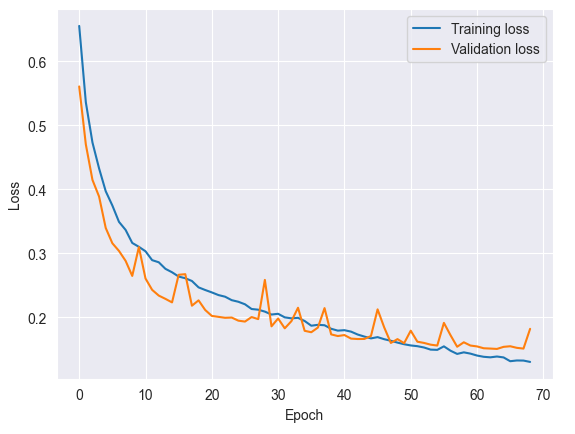
\includegraphics[width=0.75\textwidth]{epochlossgraph.png}
    \caption{Loss Graph}
    \label{fig:my_pic}
\end{figure}
\pagebreak

\subsection{(10 Puan)} \textbf{SEED=öğrenci numaranız set ettikten sonra altıncı haftada ödev olarak verdiğim gibi earlystopping'deki en iyi modeli kullanarak, Prensesi İyileştir test setinden accuracy, F1, precision ve recall değerlerini hesaplayan kodu yazın ve sonucu da aşağı yapıştırın. \%80'den fazla başarı bekliyorum test setinden. Daha düşükse başarı oranınız, nerede hata yaptığınızı bulmaya çalışın. \%90'dan fazla başarı almak mümkün (ben denedim).}

\begin{python}
from sklearn.metrics import accuracy_score, f1_score, precision_score, recall_score

model.load_state_dict(torch.load('checkpoint.pt'))

preds = []
tlabels = []
model.eval()
with torch.no_grad():
    for inputs, labels in test_loader:
        outputs = model(inputs)
        predicted = torch.round(outputs)
        preds.extend(predicted.detach().cpu().numpy())
        tlabels.extend(labels.detach().cpu().numpy())

accuracy = accuracy_score(tlabels, preds)
f1 = f1_score(tlabels, preds)
precision = precision_score(tlabels, preds)
recall = recall_score(tlabels, preds)

print(f'Accuracy: {accuracy:.4f}')
print(f'F1 score: {f1:.4f}')
print(f'Precision: {precision:.4f}')
print(f'Recall: {recall:.4f}')
\end{python}

Accuracy: 0.9534
F1 score: 0.9531
Precision: 0.9632
Recall: 0.9433

\subsection{(5 Puan)} \textbf{Tüm kodların CPU'da çalışması ne kadar sürüyor hesaplayın. Sonra to device yöntemini kullanarak modeli ve verileri GPU'ya atıp kodu bir de böyle çalıştırın ve ne kadar sürdüğünü hesaplayın. Süreleri aşağıdaki tabloya koyun. GPU için Google Colab ya da Kaggle'ı kullanabilirsiniz, iki ortam da her hafta saatlerce GPU hakkı veriyor.}

\begin{table}[ht!]
    \centering
    \caption{Kodun Çalışma Zamanı}
    \begin{tabular}{c|c}
        Ortam & Süre (saniye) \\\hline
        CPU & 19.07 \\
        GPU & 17.43 \\
    \end{tabular}
    \label{tab:my_table}
\end{table}

\subsection{(3 Puan)} \textbf{Modelin eğitim setine overfit etmesi için elinizden geldiği kadar kodu gereken şekilde değiştirin, validasyon loss'unun açıkça yükselmeye başladığı, training ve validation loss'ları içeren figürü aşağı koyun ve overfit için yaptığınız değişiklikleri aşağı yazın. Overfit, tam bir çanak gibi olmalı ve yükselmeli. Ona göre parametrelerle oynayın.}

Epoch'u arttırıp 1500 yaptım ve learning rate'i arttırıp 0.002 yaptım.

% Figür aşağı

\begin{figure}[ht!]
    \centering
    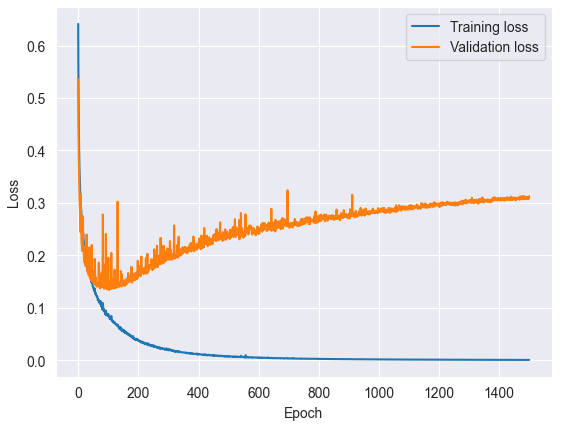
\includegraphics[width=0.75\textwidth]{overfit.png}
    \caption{Overfit}
    \label{fig:my_pic}
\end{figure}


\subsection{(2 Puan)} \textbf{Beşinci soruya ait tüm kodların ve cevapların olduğu jupyter notebook'un Github linkini aşağıdaki url'e koyun.}

\url{https://github.com/mozancetin/Yapay-Sinir-Aglari/blob/main/Soru%205%20ve%206}

\section{(Toplam 10 Puan)} \textbf{Bir önceki sorudaki Prensesi İyileştir problemindeki yapay sinir ağınıza seçtiğiniz herhangi iki farklı regülarizasyon yöntemi ekleyin ve aşağıdaki soruları cevaplayın.} 

\subsection{(2 puan)} \textbf{Kodlarda regülarizasyon eklediğiniz kısımları aşağı koyun:} 

\begin{python}
# Ilk degisiklik burada class icerisinde dropout ve batchnorm1d eklendi
class MLP(nn.Module):
    def __init__(self, input_size, hidden_size1, hidden_size2, output_size):
        super(MLP, self).__init__()
        self.fc1 = nn.Linear(input_size, hidden_size1)
        self.fc2 = nn.Linear(hidden_size1, hidden_size2)
        self.fc3 = nn.Linear(hidden_size2, output_size)
        self.relu = nn.ReLU()
        self.sigmoid = nn.Sigmoid()
        self.dropout = nn.Dropout(p=0.1)
        self.bn1 = nn.BatchNorm1d(hidden_size1)
        self.bn2 = nn.BatchNorm1d(hidden_size2)

    def forward(self, x):
        output1 = self.bn1(self.dropout(self.relu(self.fc1(x))))
        output2 = self.bn2(self.dropout(self.relu(self.fc2(output1))))
        output3 = self.sigmoid(self.fc3(output2))
        return output3
        
# Ikinci degisiklik optimizer alanında weight_decay eklendi
l2_lambda = 0.01
optimizer = optim.SGD(model.parameters(), lr=learning_rate, weight_decay=l2_lambda)
\end{python}

\subsection{(2 puan)} \textbf{Test setinden yeni accuracy, F1, precision ve recall değerlerini hesaplayıp aşağı koyun:}

Accuracy: 0.9301
F1 score: 0.9291
Precision: 0.9465
Recall: 0.9124

\subsection{(5 puan)} \textbf{Regülarizasyon yöntemi seçimlerinizin sebeplerini ve sonuçlara etkisini yorumlayın:}

Dropout, aşırı öğrenmeye karşı koruma sağlıyor. Bunun da modelin test verileri üzerinde daha iyi performans göstermesine yardımcı olacağını düşündüm.
BatchNormalization veri dağılımının daha iyi olmasını sağlıyor. Bu, modelin daha hızlı ve daha düşük bir hata oranıyla eğitilmesine yardımcı oluyor.
L2 Regularization, aşırı uyumu önleyerek modelin genelleştirilebilirliğini artırır. Bu, modelin daha iyi test sonuçları vermesine yardımcı oluyor.

Etkilerine gelecek olursak grafik bayağı değişti val loss bi artıp bir azalır şekilde grafik çizmeye başladı. Accuracy, F1, precision ve recall değerleri kötü etkilendi.

\subsection{(1 puan)} \textbf{Sonucun github linkini  aşağıya koyun:}

\url{https://github.com/mozancetin/Yapay-Sinir-Aglari/blob/main/Soru%205%20ve%206/Soru%206.ipynb}

\end{document}